\documentclass{beamer}
\usepackage{listings}
\usepackage{mathtools}
\usepackage{tikz}
\usetikzlibrary{arrows,shapes.gates.logic.US,shapes.gates.logic.IEC,calc}
\usepackage{xcolor}
\usepackage{circuitikz}
\usepackage{tkz-euclide}
\lstset{
%language=C,
frame=single, 
breaklines=true,
columns=fullflexible
}
\usepackage{subcaption}
\usepackage{url}
\usepackage{tikz}
\usepackage{tkz-euclide} % loads  TikZ and tkz-base
%\usetkzobj{all}
\usetikzlibrary{calc,math}
\usepackage{float}
\newcommand\norm[1]{\left\lVert#1\right\rVert}
\renewcommand{\vec}[1]{\mathbf{#1}}
\usepackage[export]{adjustbox}
\usepackage[utf8]{inputenc}
\usepackage{amsmath}
\usetheme{Boadilla}
\title{Joint and Marginal Probability Analysis of Markov Random Field Networks for Digital Logic Circuits}
\author{Perambuduri Srikaran}
\institute{IITH AI}
%\date{May 9, 2021}
\begin{document}
\providecommand{\pr}[1]{\ensuremath{\Pr\left(#1\right)}}
\providecommand{\qfunc}[1]{\ensuremath{Q\left(#1\right)}}
\providecommand{\sbrak}[1]{\ensuremath{{}\left[#1\right]}}
\providecommand{\lsbrak}[1]{\ensuremath{{}\left[#1\right.}}
\providecommand{\rsbrak}[1]{\ensuremath{{}\left.#1\right]}}
\providecommand{\brak}[1]{\ensuremath{\left(#1\right)}}
\providecommand{\lbrak}[1]{\ensuremath{\left(#1\right.}}
\providecommand{\rbrak}[1]{\ensuremath{\left.#1\right)}}
\providecommand{\cbrak}[1]{\ensuremath{\left\{#1\right\}}}
\providecommand{\lcbrak}[1]{\ensuremath{\left\{#1\right.}}
\providecommand{\rcbrak}[1]{\ensuremath{\left.#1\right\}}}
\providecommand{\brak}[1]{\ensuremath{\left(#1\right)}}
\begin{frame}
\titlepage
\end{frame}
\section{Authors}
\begin{frame}
\frametitle{Authors and other details}
\begin{block}{Authors}
\begin{itemize}
    \item Jahanzeb Anwer
    \item Usman Khalid
    \item Narinderjit Singh
    \item Nor H. Hamid
    \item Vijanth S. Asirvadam
\end{itemize}
\end{block}
\begin{block}{Conference}
2010 International Conference on Intelligent and Advanced Systems, Malaysia
\end{block}
\end{frame}
\section{Introduction}
\begin{frame}
\frametitle{Introduction}
\begin{flushleft}
\begin{itemize}
    \item Nanoscale electronic circuits are suffering from both manufacturing defects and transient faults.
    \item Since, the integrated circuits are scaling to nano-level, they are expected to face high computing errors.
    \item Markov Random Field modelling is one approach to achieve noise-tolerance.
\end{itemize}
\end{flushleft}
\end{frame}
\section{Cliques}
\begin{frame}[fragile]
\frametitle{Cliques}
\begin{flushleft}
\begin{itemize}
    \item A clique is a complete subgraph of a given graph.\\
    \item A maximal clique is a clique that cannot be extended by including one more adjacent vertex.
\end{itemize}
\begin{figure}[h]
\centering
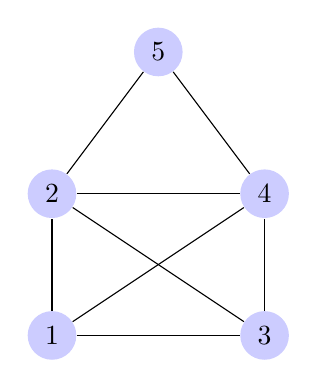
\begin{tikzpicture}[scale=.9,auto=center,every node/.style={circle,fill=blue!20}]
  \node (a1) at (0,1) {1};  
  \node (a2) at (0,3) {2};
  \node (a3) at (3,1) {3};  
  \node (a4) at (3,3) {4};
  \node (a5) at (1.5,5) {5};
  
  \draw (a1) -- (a2);
  \draw (a1) -- (a3);
  \draw (a3) -- (a4);
  \draw (a4) -- (a2);
  \draw (a3) -- (a2);
  \draw (a1) -- (a4);
  \draw (a5) -- (a2);
  \draw (a5) -- (a4);
\end{tikzpicture}
\caption*{\textbf{Markov network}}
\end{figure}
\end{flushleft}
\end{frame}
\section{Joint Probabilty of MRF}
\begin{frame}
\frametitle{Joint Probability of MRF}
\begin{flushleft}
\begin{block}{Gibbs distribution}
A Gibbs distribution on the graph G takes the form:
\begin{align}
    \pr{X} &= \frac{1}{Z}\prod_{c\in C}\phi_c(x_c)\\
    \phi_c(x_c) &= e^{-\frac{U_c(x_c)}{kT}}
\end{align}
\end{block}
\begin{itemize}
    \item The Hammersley-Clifford theorem states that the joint probability distribution of any MRF can be written as a Gibbs distribution, and furthermore that for any Gibbs distribution there exists an MRF for which it is the joint. 
\end{itemize}
\end{flushleft}
\end{frame}
\section{Marginal Probability}
\begin{frame}
\frametitle{Marginal Probability}
\begin{flushleft}
\begin{itemize}
    \item We fix the value of one or more variables and sum it over non-fixed variables.
\end{itemize}
\begin{align}
    \pr{X=x} &= \sum_{y}\pr{X=x,Y=y}\\ 
    &= \sum_{y}\pr{X=x | Y=y}\pr{Y=y}
\end{align}
\end{flushleft}
\end{frame}
\section{Computing Joint Probability}
\subsection{Circuit}
\begin{frame}
\frametitle{Computing Joint Probability}
\begin{flushleft}
\begin{figure}[h]
\centering
\begin{tikzpicture}[label distance=2mm]
\node (x0) at (0,5) {$x_0$};
\node (x1) at (0,4.5) {$x_1$};
\node (x2) at (0,2) {$x_2$};
\node (x3) at (0,0) {$x_3$};
\node (x4) at (1.75,0) {$x_4$};
\node (x5) at (4,2.1) {$x_5$};
\node (x6) at (8.2,5) {$x_6$};

\node[not gate US, draw] at ($(x3)+(1,0)$)(Not1){};
\node[nor gate US, draw, logic gate inputs=nn, anchor=input 1] at ($(x2)+(3,0)$) (Nor1) {};
\node[nand gate US, draw, logic gate inputs=nnn, anchor= input 1] at ($(7,5)$) (Nand1) {};
\node[not gate US, draw] at ($(Nand1)+(2,0)$)(Not2){};

\draw (x3) -- (Not1.input);
\draw (x2) -- (Nor1.input 1);
\draw (Not1.output) |- (Nor1.input 2);
\draw (x0) -- (Nand1.input 1);
%\draw (Xor1.output) -- ([xshift=0.5cm]Xor1.output) |- (And1.input 2);
\draw (x1) -- ([xshift=2.5cm]x1) |- (Nand1.input 2);
\draw (Nor1.output) -- ([xshift=2.5cm]Nor1.output) |- (Nand1.input 3);
\draw (Nand1.output) -- (Not2.input);
\draw (Not2) -- ([xshift=0.5cm]Not2.output) node[right] {$x_7$};
\end{tikzpicture}
\caption*{\textbf{M3 module of C432 Interrupt Controller}}
\end{figure}
\end{flushleft}
\end{frame}
\subsection{Dependence Graph}
\begin{frame}
\frametitle{Computing Joint Probability (contd...)}
\begin{flushleft}
\begin{figure}[h]
\centering
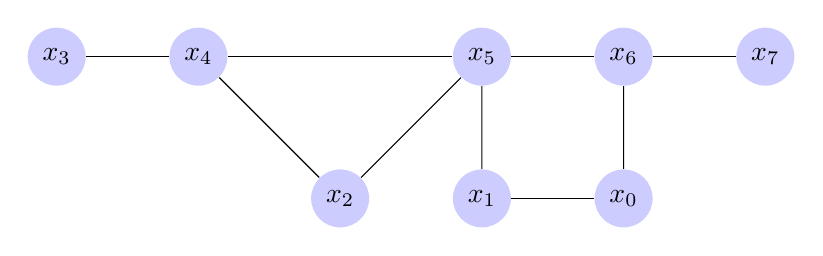
\begin{tikzpicture}[scale=.9,auto=center,every node/.style={circle,fill=blue!20}]
  \node (x3) at (0,2) {$x_3$};
  \node (x4) at (2,2) {$x_4$};
  \node (x2) at (4,0) {$x_2$};
  \node (x5) at (6,2) {$x_5$};
  \node (x1) at (6,0) {$x_1$};
  \node (x6) at (8,2) {$x_6$};
  \node (x0) at (8,0) {$x_0$};
  \node (x7) at (10,2) {$x_7$};
  
  \draw (x3) -- (x4);
  \draw (x4) -- (x5);
  \draw (x4) -- (x2);
  \draw (x2) -- (x5);
  \draw (x5) -- (x1);
  \draw (x5) -- (x6);
  \draw (x1) -- (x0);
  \draw (x0) -- (x6);
  \draw (x6) -- (x7);
\end{tikzpicture}
\caption*{\textbf{Dependence graph of the test circuit}}
\end{figure}
Cliques: \cbrak{x_3,x_4},\cbrak{x_2,x_4,x_5},\cbrak{x_0,x_1,x_5,x_6},\cbrak{x_6,x_7}
\end{flushleft}
\end{frame}
\subsection{Logic Compatibility Function}
\begin{frame}
\frametitle{Computing Joint Probability (contd...)}
\begin{flushleft}
\begin{center}
\begin{table}{}
\begin{tabular}{|l|l|l|l|l|}
\hline
$x_0$ & $x_1$ & $x_5$ & $x_6$ & f \\ \hline
0 & 0 & 0 & 1 & 1 \\ \hline
0 & 0 & 0 & 0 & 0 \\ \hline
0 & 0 & 1 & 1 & 1 \\ \hline
0 & 0 & 1 & 0 & 0 \\ \hline
0 & 1 & 0 & 1 & 1 \\ \hline
0 & 1 & 0 & 0 & 0 \\ \hline
0 & 1 & 1 & 1 & 1 \\ \hline
0 & 1 & 1 & 0 & 0 \\ \hline
\end{tabular}
\hspace{3em}
\begin{tabular}{|l|l|l|l|l|}
\hline
$x_0$ & $x_1$ & $x_5$ & $x_6$ & f \\ \hline
1 & 0 & 0 & 1 & 1 \\ \hline
1 & 0 & 0 & 0 & 0 \\ \hline
1 & 0 & 1 & 1 & 1 \\ \hline
1 & 0 & 1 & 0 & 0 \\ \hline
1 & 1 & 0 & 1 & 1 \\ \hline
1 & 1 & 0 & 0 & 0 \\ \hline
1 & 1 & 1 & 0 & 1 \\ \hline
1 & 1 & 1 & 1 & 0 \\ \hline
\end{tabular}
\caption*{\textbf{Logic Compatibility Function for NAND}}
\end{table}
\end{center}
\end{flushleft}
\end{frame}
\subsection{Calculating Clique Energy}
\begin{frame}
\frametitle{Computing Joint Probability (contd...)}
\begin{flushleft}
We will compute the clique energy function for \cbrak{x_0,x_1,x_5,x_6}
\begin{multline}
U_c = -\sum\lbrak{\text{Valid minterms}} \brak{f=1} \text{in the Logic}\\\rbrak{\text{Compatibility Function}}\label{eq:4}
\end{multline}
\begin{multline}
= -\lsbrak{x_0'x_1'x_5'x_6 + x_0'x_1'x_5x_6 + x_0'x_1x_5'x_6 + x_0'x_1x_5x_6 +}\\ \rsbrak{x_0x_1'x_5'x_6 + x_0x_1'x_5x_6 + x_0x_1x_5x_6'} \label{eq:5}
\end{multline}
\begin{flalign}
\phantom{aa}= 2x_0x_1x_5x_6 - x_0x_1x_5 - x_6&&
\end{flalign}
\end{flushleft}
\end{frame}
\begin{frame}
\frametitle{Computing Joint Probability (contd...)}
\begin{flushleft}
\begin{center}
\begin{table}[h]
\caption*{\textbf{Clique energy functions for NOT and NOR gates}}
\begin{tabular}{|l|l|}
\hline
NOT 1 & $2x_3x_4 - x_3 - x_4$ \\ \hline
NOR & $x_2x_4 + 2x_4x_5 + 2x_2x_5 - 2x_2x_4x_5 - x_2 - x_4 - x_5$ \\ \hline
NOT 2 & $2x_6x_7 - x_6 - x_7$ \\ \hline
\end{tabular}
\end{table}
\end{center}
Now, we will compute the joint probability
\begin{multline}
\pr{x_0,x_1,x_2,x_3,x_4,x_5,x_6,x_7} = \frac{1}{Z}\lbrak{e^{\frac{-U_c\brak{\text{NOT 1}}}{kT}} e^{\frac{-U_c\brak{\text{NAND}}}{kT}} e^{\frac{-U_c\brak{\text{NOR}}}{kT}}}\\\rbrak{e^{\frac{-U_c\brak{\text{NOT 2}}}{kT}}}
\end{multline}
\begin{align}
=\frac{1}{Z}exp\sbrak{\frac{\splitdfrac{x_2+x3+2x_4+x_5+2x_6+x_7-x_2x_4-2x_2x_5-2x_3x_4}{-2x_4x_5-2x_6x_7+x_0x_1x_5+2x_2x_4x_5-2x_0x_1x_5x_6}}{kT}}
\end{align}
\end{flushleft}
\end{frame}
\subsection{Design Principle}
\begin{frame}
\frametitle{Computing Joint Probability (contd...)}
\begin{flushleft}
\begin{itemize}
\item Following the joint probability calculation, we need to find the node label combinations that maximize its value.
\item The maximum value is $\frac{1}{Z}e^{\frac{4}{kT}}$. There are 16 node label combinations.
\item These 16 combinations are same as the circuit's truth table, which shows that joint probability is maximum only for correct logic combinations.
\item For the rest of the combinations, the joint probability is lower.
\end{itemize}
\begin{block}{Design Principle of Joint Probability}
For perfect logic operation of a circuit, we need to design our circuit such that joint probability of the circuit remains maximum at all times.
\end{block}
\end{flushleft}
\end{frame}
\section{Computing Marginal Probability}
\subsection{Assigning PDF}
\begin{frame}
\frametitle{Computing Marginal Probability}
\begin{flushleft}
\begin{itemize}
    \item For computing the probability of the (intermediate and output) nodes, we will use the belief propagation algorithm.
    \item We will assign PDFs to all inputs and cliques.
\end{itemize}
\begin{align}
    \pr{x_7} = f_0f_1f_2f_3f_4f_5f_6f_7
\end{align}
\begin{center}
\begin{table}[h]
\caption*{\textbf{PDFs for Inputs and Cliques}}
\begin{tabular}{|l|l|l|l|}
\hline
Input & PDF & Clique & PDF \\ \hline
$x_0$ & $f_0$\brak{s_0} & \cbrak{x_3,x_4} & $f_4$\brak{x_3,x_4} \\ \hline
$x_1$ & $f_1$\brak{s_1} & \cbrak{x_2,x_4,x_5} & $f_5$\brak{x_2,x_4,x_5}  \\ \hline
$x_2$ & $f_2$\brak{s_2} & \cbrak{x_0,x_1,x_5,x_6} & $f_6$\brak{x_0,x_1,x_5,x_6} \\ \hline
$x_3$ & $f_3$\brak{s_3} & \cbrak{x_6,x_7} & $f_7$\brak{x_6,x_7} \\ \hline
\end{tabular}
\end{table}
\end{center}
\end{flushleft}
\end{frame}
\subsection{BFA Step 1}
\begin{frame}
\frametitle{Computing Marginal Probability (contd...)}
\begin{flushleft}
Step 1: (Eliminating $x_3$)
\begin{align}
    \pr{x_4} &= \sum_{x_3 \in \cbrak{0,1}}\frac{1}{Z_1} e^{-\frac{U_c\brak{\text{NOT 1}}}{kT}}\\
    &= \frac{1}{Z_1}\brak{e^{\frac{x_4}{kT}} + e^{\frac{1 - x_4}{kT}}}\\
    &= f_8\brak{x_4}\\
    \pr{x_7} &= f_0f_1f_2f_5f_6f_7f_8
\end{align}
\end{flushleft}
\end{frame}
\subsection{BFA Step 2}
\begin{frame}
\frametitle{Computing Marginal Probability (contd...)}
\begin{flushleft}
Step 2: (Eliminating $x_2$)
\begin{align}
    \pr{x_5|x_4} &= \sum_{x_2 \in \cbrak{0,1}} \frac{1}{Z_2}e^{-\frac{U_c\brak{\text{NOR}}}{kT}}\\
    &= \frac{1}{Z_2}\brak{e^{\frac{x_4+x_5-2x_4x_5}{kT}} + e^{\frac{1-x_5}{kT}}}\\
    &= f_9\brak{x_4,x_5}\\
    \pr{x_7} &= f_0f_1f_6f_7f_8f_9
\end{align}
\end{flushleft}
\end{frame}
\subsection{Graphs}
\begin{frame}
\frametitle{Computing Marginal Probability (contd...)}
\begin{flushleft}
\begin{figure}[h]
    \centering
    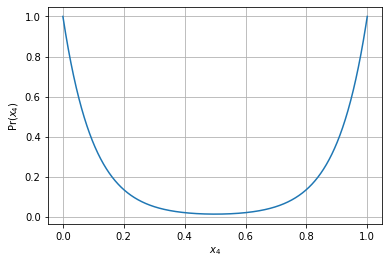
\includegraphics[width=8cm]{ProbX4.png}
    \caption{{Plot of probability of $x_4$ against $x_4$}}
    \label{fig:plot}
\end{figure}
\end{flushleft}
\end{frame}
\begin{frame}
\frametitle{Computing Marginal Probability (contd...)}
\begin{flushleft}
\begin{figure}[h]
    \centering
    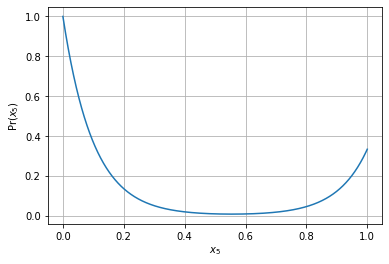
\includegraphics[width=8cm]{ProbX5.png}
    \caption{{Plot of probability of $x_5$ against $x_5$}}
    \label{fig:plot}
\end{figure}
\end{flushleft}
\end{frame}
\begin{frame}
\frametitle{Computing Marginal Probability (contd...)}
\begin{flushleft}
\begin{figure}[h]
    \centering
    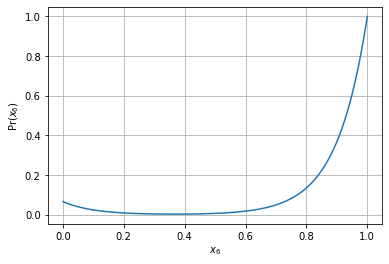
\includegraphics[width=8cm]{ProbX6.png}
    \caption{{Plot of probability of $x_6$ against $x_6$}}
    \label{fig:plot}
\end{figure}
\end{flushleft}
\end{frame}
\begin{frame}
\frametitle{Computing Marginal Probability (contd...)}
\begin{flushleft}
\begin{figure}[h]
    \centering
    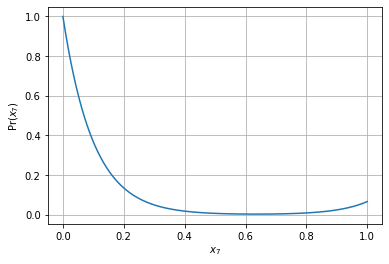
\includegraphics[width=8cm]{ProbX7.png}
    \caption{{Plot of probability of $x_7$ against $x_7$}}
    \label{fig:plot}
\end{figure}
\end{flushleft}
\end{frame}
\begin{frame}
\frametitle{Computing Marginal Probability (contd...)}
\begin{flushleft}
\begin{figure}[h]
    \centering
    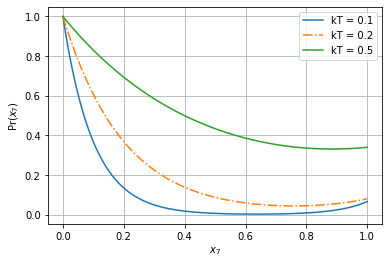
\includegraphics[width=8cm]{Comparsion.png}
    \caption{{Plot of probability of $x_7$ for different values of T}}
    \label{fig:plot}
\end{figure}
\end{flushleft}
\end{frame}
\subsection{Design Principle}
\begin{frame}
\frametitle{Computing Marginal Probability (contd...)}
\begin{flushleft}
\begin{block}{Design Principle of Marginal Probability}
The key to design a fault-tolerant circuit is to ensure a good heat removal system for the integrated circuit which would make the probability of intermediate states between ‘0’ and ‘1’ close to zero and maintain sufficient noise margin as well.
\end{block}
\end{flushleft}
\end{frame}
\end{document}